\section{Related Work}
\label{sec:related_work}

Approximating geodesic paths is a widely studied area of research, and many methods to do so have been developed. For a comprehensive survey on this subject, please refer to \citet{crane2020survey}. Our work is specifically inspired from the ISOMAP method \citep{tenenbaum2000global}, a dimensionality reduction method which approximates geodesic paths on a manifold. However, our method differs from ISOMAP in that we weight our graph not using euclidean distance, but the norms of a model's gradients. Our aim is indeed not to model the input space, but to explain a neural network by building paths avoiding high-gradients regions.

As mentioned in Section \ref{sec:experiments}, the idea of using a $k$NN algorithm to avoid computing gradients on out of distribution data points has also been used in Enhanced Integrated Gradients \citet{jha2020enhanced}. However, this method creates a path which is model agnostic, as it does not necessarily avoid high gradients regions. As a result, it can lead to significant artefacts which do not reflect the model's behaviour. To support this argument, we provide an example where this method fails on the half-moons datasets (Figure \ref{fig:enhanced_ig}). 

\begin{figure}[ht]
\vskip -0.2in
\begin{center}
\centerline{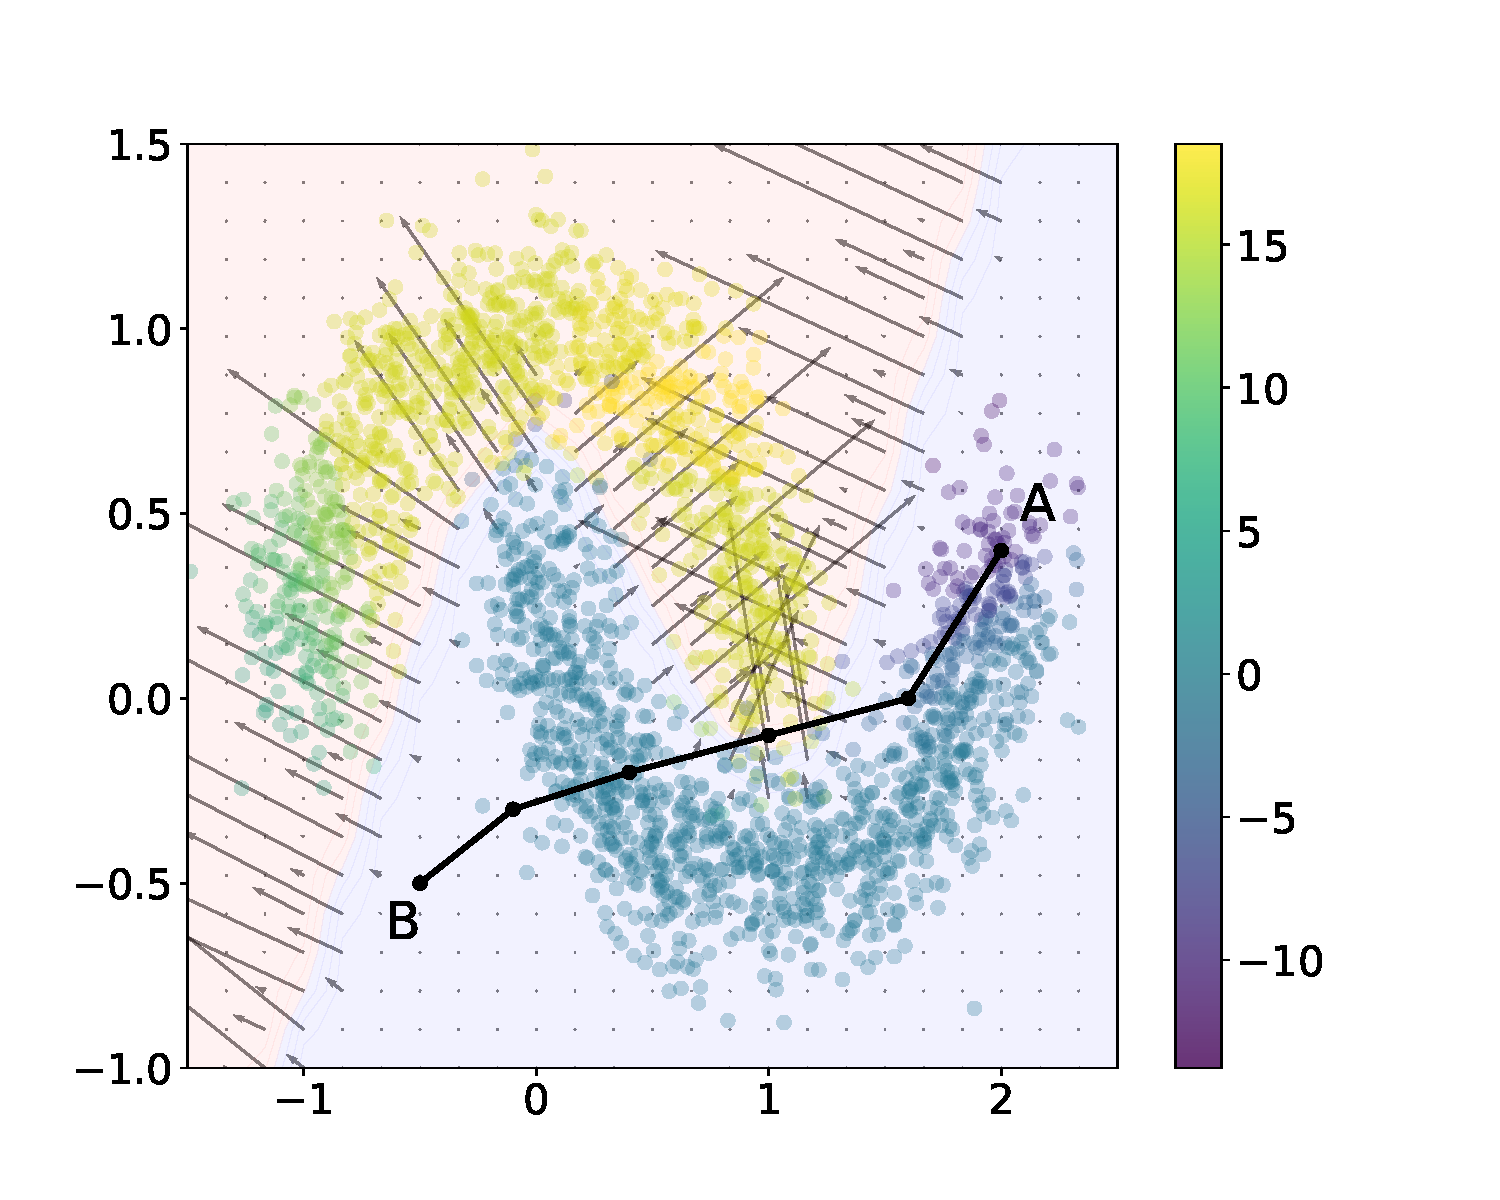
\includegraphics[width=\columnwidth]{figures/enhanced_ig_y.pdf}}
\caption{\textbf{Enhanced IG attributions.} Enhanced IG computes a $k$NN algorithm, uses Dijsktra to find the shortest path between an input and a reference baseline, and computes gradients along this path. However, this method is model agnostic and can as a result cross a high gradients region, which is the case in this example, between the input A and the baseline B. Input A therefore has a high attribution which does not reflect the model's true behavior. In this example, the noise is $\mathcal{N}(0, 0.15)$.}
\label{fig:enhanced_ig}
\end{center}
\vskip -0.2in
\end{figure}

The idea of adapting the path according to the model has be proposed by \citet{kapishnikov2021guided}, calling their method Guided Integrated Gradients. Their method computes this path greedily by selecting around 10\% of the features that have the lowest absolute value of the partial derivatives, and switching these features from the baseline's values to the input's values. However, as the authors indicate, such method can create out of distribution data points, with part of their features either matching the input or the baseline. As a result, they add a hyperparameter K, which forces the path to go through K points along the straight line between the input and the baseline. 
We argue, however, that, by directly approximating the path of least resistance, our method is more principled compared to Guided IG. In Guided IG, it is not clear how to choose the value of K: a too low value could create out of distribution samples, while a too high one would force the path to be close to the straight line and potentially cross high gradients regions. It is similarly not clear why switching 10\% of the features, and how to tune this hyperparamer. On the other hand, we argue that Geodesic IG does not have this issue. It has indeed two hyperparamers: the number of points used to approximate the geodesic path, and the number k of nearest neighbours. Yet, the performance of Geodesic IG should improve when both hyperparamers values increase, as, when more points or more neighbours are used, the approximation of the geodesic path should improve. Increasing these values would, however, require more computing and performance needs to be balanced with the amount of compute available.